\documentclass{beamer}
\beamertemplatenavigationsymbolsempty
\usetheme{Rochester}
\usecolortheme{beaver}
%\usepackage[utf8]{inputenc}
\usepackage[english]{babel}
\parindent=0.pt
\usepackage{amsmath}
\usepackage{graphicx}
\usepackage{verbatim}
\usepackage{tikz}
\usepackage{csquotes}
\usepackage[backend=biber,
style=phys,
citestyle=authoryear
]{biblatex}
\addbibresource{biblio.bib} 
\usepackage[export]{adjustbox}
\usefonttheme[onlymath]{serif}
\newcommand{\R}{\mathbb{R}}
\DeclareMathOperator\supp{supp}
\DeclareMathOperator\shannon{H}
\renewcommand{\qedsymbol}{\includegraphics[width=0.6in, right]{QED Gregory.png}}
\graphicspath{{./Images}/}


\title{Thermodynamic Costs of Turing Machines \parencite{Kolchinsky_2020}}
\author{Daniel Briseno}


\begin{document}
\frame{\titlepage}
%Re-introduce context of the paper and the paper's main results

\begin{frame}{Context of the Paper}
\begin{block}{Prior work on Thermodynamics of Information Processing}
\begin{itemize}
    \item Landauer cost of erasing a bit: $kT\ln2$ (1961)
    \item Logically reversible computations can be performed with no heat or entropy production (1973)
    \item Informal argument for minimum cost of $x\mapsto y$ (1989 - 2019)
    \item Development of non-equilibrium statistical physics
    \begin{itemize}
        \item Trajectory-based and stochastic thermodynamics (2013-2015)
    \end{itemize}
    \item Thermodynamic costs of specific implementations of Turing Machines (TM)(2015-2019)
    
    
\end{itemize}
\end{block}
\end{frame}


\begin{frame}{Purpose of the Paper}
    \begin{block}{Thermodynamic costs of computation}
    \begin{itemize}
        \item Extends results to general class of TM
        \item Analyzes the thermodynamic costs of $f:\mathbb{N} \nrightarrow \mathbb{N}$ on a physical implementation of a TM $M$
        \item Logical properties of $f$ and $M$ impose constraints on thermodynamic costs.
        \item Result might generalize to any implementation of a TM
        
    \end{itemize}
    \end{block}
\end{frame}

%Recap of Background info


%%%%%%%%%%%%%%%%%%% CS Background
%TM Visual
\begin{frame}{Background -- Computer Science}
 \begin{block}{Turing Machines}
        \begin{figure}
            \centering
            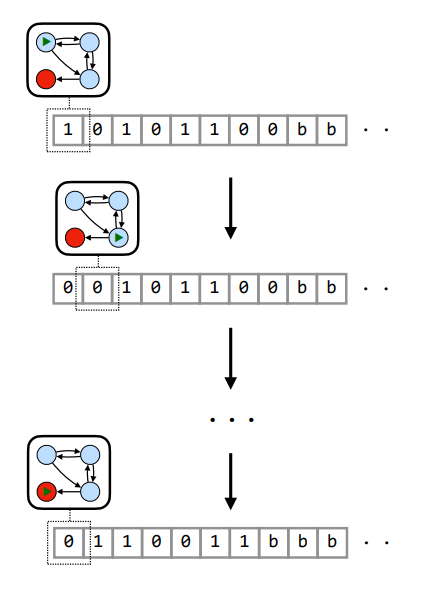
\includegraphics[height=5cm]{TM.png}
            \caption{Graphical representation of a TM}
            \label{fig:TM}
        \end{figure}
    \end{block}
\end{frame}

%Additional Assumptions on TM
\begin{frame}{Background -- Computer Science}
    \begin{block}{Additional Assumptions on TM $M$}
    \begin{enumerate}
        \item $\Sigma = \{0,1,b\}$
        \item If and when $M$ halts on an input, the tape will contain an output string $s\in \{0,1\}^*$ followed by all blank symbols, and the pointer will be set to the start of the tape.
    \end{enumerate}
    Assumptions do not affect the computational capabilities of $M$.
    \end{block}
\end{frame}

% TM as partial functions and UTMs
\begin{frame}{Background -- Computer Science}
    \begin{block}{Turing Machines as Partial Functions}
    Any computation performed by a TM $M$ can be represented as
    \begin{equation*}
        \phi_M:\{0,1\}^* \nrightarrow \{0,1\}^*
    \end{equation*}
    and $\phi_M(x) = y$ indicates that $M$ started with input program $x$ yields the output string $y$.
    \end{block}
    \begin{block}{Universal TM}
    There exist Universal Turing Machines (UTM) such that given a UTM $U$ and any TM $M$, there exists an interpreter program $\sigma_{U,M}$ such that
    \begin{equation*}
        \phi_U(\sigma_{U,M},x) = \phi_M(x)
    \end{equation*}
    \end{block}
\end{frame}

\begin{frame}{Background -- Computer Science}
    \begin{block}{Computability}
    \begin{itemize}
        \item Church Turing Thesis: A function can be calculated by a sequence of formal operations if and only if it is computable by a Turing Machine.
       \item Physical Church Turing Thesis: Any function implemented by a physical process can also be implemented by a Turing Machine
    \end{itemize}
    \end{block}
\end{frame}

%%%%%%%%%%%%%%%%%%%% AIT background 
% Kolomogorov Complexity Defintion
\begin{frame}{Background -- Algorithmic Information Theory}
\begin{block}{Kolmogorov Complexity}
The Kolmogorov complexity $K_U$ of a bitstring $x$ is the length of the shortest input program that when given to a UTM $U$ can produce $x$ as an output:
\begin{equation*}
    K_U(x) :=\min_{z:\phi_U(z) = x}\ell(z)
\end{equation*}
\begin{itemize}
    \item Measure of amount of information in $x$
\end{itemize}
\end{block}
\end{frame}

%Variations on Kolomogorov Complexity
\begin{frame}{Background -- Algorithmic Information Theory}
    \begin{block}{Kolmogorov Complexity of Bitstring $x$}
    \begin{equation*}
        K_U(x) :=\min_{z:\phi_U(z) = x}\ell(z)
    \end{equation*}
    \end{block}
    \begin{block}{Kolmogorov Complexity of a Computable Function $f$}
    \begin{equation*}
        K_U(f) := \min_{M:\phi_M = f} \ell(\sigma_{U,M})
    \end{equation*}
    \end{block}
    \begin{block}{Conditional Kolmogorov Complexity of $x$ Given Bitstring $y$}
\begin{equation*}
    K_U(x|y) = \min_{z:\phi_U(z,y) = x} \ell(z)
\end{equation*}
\end{block}
\end{frame}

%Invariance Theorem
\begin{frame}{Background -- Algorithmic Information Theory}
    \begin{block}{Invariance Theorem}
    For distinct UTM $U$, $U'$:
        \begin{equation*}
            K_{U'}(x) = K_U(x) + O(1)
        \end{equation*}
        Thus, $U$ is usually omitted and we write $K(x)$ for Kolmogorov complexity of $x$
    \end{block}
\end{frame}

%%%%%%%%%%%%% Input Distributions
\begin{frame}{Background -- Input Distributions}
\begin{block}{Coin-Flipping Distribution}
\begin{itemize}
    \item Input string $x$ as random variable with probability distribution $p_X$
    \item Important example: coin flipping distribution of TM $M$
    \begin{equation*}
        m_X^\text{coin}(x) := \begin{cases} 2^{-\ell(x)} &\text{if $x\;\in$ dom $\phi_M$}\\ 0 &\text{otherwise}\end{cases}
    \end{equation*}
    \item With normalizing constant $\Omega_M :=\sum_{x\in\text{ dom }\phi_M} 2^{-\ell(x)}$
    \begin{equation*}
        p_X^\text{coin}(x) = m_X^\text{coin}(x)/\Omega_M
    \end{equation*}
\end{itemize}
\end{block}
\end{frame}


%%%%%%%%%%%% Entropy
%Definition of Entropy
\begin{frame}{Background -- Entropy}
    \begin{block}{Shannon Entropy of Distribution $p_X$}
    \begin{equation*}
    S(p_X) = - \sum_{x\in X} p_X(x)\ln [p_X(x)]    
    \end{equation*}
    \begin{itemize}
        \item Measure of amount of information in $p_X$
        \item $-\ln[p_X(x)]$: ``surprisal", how unexpected, and hence informative, is $x$?
        \item $p_X(x)$: how often do we receive surprise $\ln p_X$
    \end{itemize}
    \end{block}
\end{frame}

%Entropy Production
\begin{frame}{Background -- Entropy}
    \begin{block}{Entropy Production (EP)}
    The expected EP, written $\Sigma (p_X)$ of a physical process with initial state distribution $p_X$ and final state distribution $p_Y$ is:
    \begin{align*}
        \Sigma (p_X) &= S(p_Y) - S(p_X) + \langle Q \rangle_{p_X}/kT
    \end{align*}
    Thermodynamically reversible processes have $\Sigma (p_X)=0$. EP is always nonnegative.
    \end{block}
\end{frame}



%Introduce System under study
\begin{frame}{Physical Setup}
\begin{block}{Physical System Under Consideration}
\begin{itemize}
	\item Countable state-space $\mathcal{X}$
	\item Connected to a work reservoir
	\item Connected to heat bath at temperature $T$
	\begin{itemize}
		\item Bath in a Boltzmann distribution
	\end{itemize}
	\item System evolves according to driving protocol during time interval $[0,t_f]$
\end{itemize}
The heat function $Q(x)$ is the expected thermal energy transferred from the system to the heat bath.
\end{block}
\end{frame}
\begin{frame}{Physical Setup}

    \begin{figure}
            \centering
            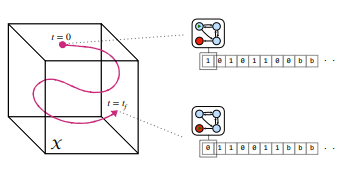
\includegraphics{System.png}
            \label{fig:system_visual}
        \end{figure}
\end{frame}

\begin{frame}{Physical Setup}
\begin{block}{System under consideration}
The joint Hamiltonian of the system is
\begin{equation*}
    H_X^t(x) + H_B(b) + H_{\text{int}}(x,b)
\end{equation*}
If $p_B(b)$ is the initial distribution of the bath and $p'_{B|X}$ is the final distribution, then:
\begin{equation*}
    Q(x) = \langle H_B \rangle_{p'_{B|x}} - \langle H_B \rangle_{p_B}
\end{equation*}
\end{block}
\end{frame}






%Introduce Proposition 1

%Formal definitions for Realization of a TM
\begin{frame}{Realizations of a TM}
\begin{block}{Realization Formally Defined}
{\footnotesize
	\begin{itemize}
		\item Let $p_{Y|X}$ be the conditional probability distribution of the system's final state $y$ given initial state $x$
		\item A physical process is a \textbf{realization} of a partial function $f : \mathcal{X} \nrightarrow \mathcal{X}$ if
		\begin{equation*}
			p_{Y|X}(y|x) = \delta(f(x),y)
		\end{equation*}
	\end{itemize}		
}
\end{block}
\begin{block}{Realization of a TM $M$ Formally Defined}
{\footnotesize
	\begin{itemize}
		\item TM $M$ can be written as a partial function $\phi_M:\{0,1\} \nrightarrow\{0,1\}$
		\item A physical process is a realization of a TM $M$ if it is a realization of $\phi_M$
		\item A physical process is a \textbf{computable realization} if its heat map $Q(x)$ is computable
	\end{itemize}
}
\end{block}
\end{frame}


%Proposition 1
\begin{frame}{Proposition 1}
\begin{block}{Proposition Statement}
Given a countable set $\mathcal{X}$ and partial functions $f:\mathcal{X} \nrightarrow \mathcal{X}$ and $G:\mathcal{X} \nrightarrow \mathbb{R}$, the following are equivalent:
\begin{enumerate}
    \item For all $p_X$ with $\text{supp}\: p_X \subseteq \text{dom}\: f$
    \begin{equation*}
        \langle G \rangle_{p_X} + S[p_{f(X)}] - S(p_X) \ge 0
    \end{equation*}
    \item For all $y\in \text{img}\: f$
    \begin{equation*}
        \sum_{x:f(x) = y} e^{-G(x)} \le 1
    \end{equation*}
    \item There exists a realization of $f$ coupled to a heat bath at temperature $T$ whose heat function $Q$ obeys
    \begin{align*}
        Q(x)/kT &= G(x)  &&\forall x\in\text{dom}\:f
    \end{align*}
\end{enumerate}
\end{block}
\end{frame}

%Recovery of Landauer cost from Prop 1

\begin{frame}{Proposition 1}
\begin{block}{Recovering Landauer Cost From Proposition 1}
{\small
Take $x\in\{0,1\}$ to be a random bit determined by a coin toss, and $f$ as the bit-erasing operation $f(x) = 0$. Then:
\begin{align*}
    p_X(x) &= \frac{1}{2}\\
    p_{f(X)}(y) &= \begin{cases} 0 &\text{if } y=1\\ 1 &\text{if }y=0\end{cases}
\end{align*}
Then for any $G(x) = Q(x)/kT$, condition 1 implies:
\begin{align*}
    \langle G \rangle_{p_X} + S[p_{f(X)}] - S(p_X) &\ge 0\\
    \implies \langle G\rangle_{p_X} &\ge S(p_X)\\
    \implies \langle G\rangle_{p_X} &\ge \ln 2
\end{align*}
}
\end{block}
\end{frame}

\begin{frame}{Proposition 1}
\begin{block}{Recovering Landauer Cost From Proposition 1 (cont.)}
We would like to characterize the cost of an arbitrary bit deletion, so taking $G$ to be identical for inputs $\{0,1\}$
\begin{align*}
    G(x) \ge \ln 2
\end{align*}
and using equivalent condition 3 from Proposition 1 we recover the Landauer cost of a bit deletion:
\begin{align*}
    Q(x)/kT &\ge \ln 2\\
    \implies Q(x) \ge kT \ln 2
\end{align*}
\end{block}
\end{frame}


\begin{frame}{Realizations of TM}
\begin{block}{Realizations of TM Used in Analysis}
    \begin{itemize}
        \item \textbf{Coin-Flipping Realization}: thermodynamically reversible when inputs are sampled from coin-flipping distribution
        \item \textbf{Dominating Realization}: produces less heat than any computable realization of a TM
    \end{itemize}
\end{block}
\end{frame}





\end{document}